%%%%%%%%%%%%
%
% Maintenance
%
%%%%%%%%%%%%

\chapter{Maintenance}
\label{ch:maintenance}

This chapter is intended primarily for maintainers, supervisors, or team members who are responsible for keeping the repository operational over time. Normal end users do not need to perform the actions described here in order to launch and use the dashboard.

\section{What End Users Should Know}

For normal dashboard use, no data update, model retraining, or backend editing is required. If the dashboard opens and shows valid forecasts, the user can continue working without touching the repository internals.

If the dashboard fails because data or model artifacts are missing, the correct action for a normal user is to contact a maintainer rather than modifying backend files independently.

\section{What Maintainers Are Responsible For}

Maintainers may occasionally need to:

\begin{itemize}
    \item verify that the saved model files still exist,
    \item confirm that dependency installation still succeeds,
    \item refresh or repair the repository state if files become corrupted,
    \item update screenshots or documentation if the user interface changes visibly.
\end{itemize}

This chapter deliberately does not encourage casual end users to replace the CPI source file or retrain the forecasting backend without coordination.

\section{Maintainer Timeline}

Figure~\ref{fig:maintenance-timeline} shows a realistic maintainer-oriented upkeep timeline for the CPI forecasting dashboard. The intervals are designed for a project that uses monthly macroeconomic data and requires periodic validation of both the software environment and the model accuracy.

\begin{figure}[H]
    \centering
    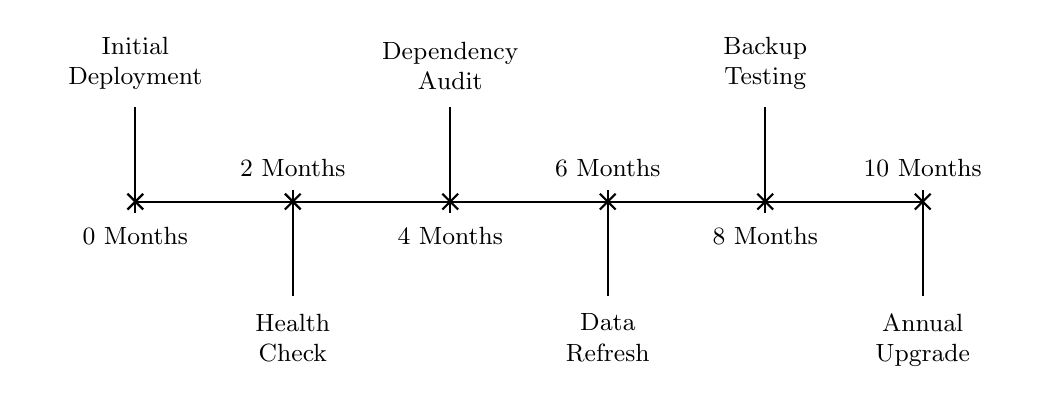
\begin{tikzpicture}[>=latex, every node/.style={font=\small}]
        % Main horizontal axis (0 to 10 months, equally spaced events)
        \draw[thick] (0,0) -- (10,0);
        
        % Tick marks and labels: all equally spaced at 2-month intervals
        % 0, 4, 8 below axis; 2, 6, 10 above axis
        \foreach \x/\label in {0/0 Months, 4/4 Months, 8/8 Months} {
            \draw[thick] (\x,0.15) -- (\x,-0.15);
            \node[below] at (\x,-0.2) {\label};
        }
        \foreach \x/\label in {2/2 Months, 6/6 Months, 10/10 Months} {
            \draw[thick] (\x,0.15) -- (\x,-0.15);
            \node[above] at (\x,0.2) {\label};
        }
        
        % X marks at all event points (equally spaced)
        \foreach \x in {0, 2, 4, 6, 8, 10} {
            \draw[thick] (\x-0.1,-0.1) -- (\x+0.1,0.1);
            \draw[thick] (\x-0.1,0.1) -- (\x+0.1,-0.1);
        }
        
        % Event above axis: Initial Deployment at 0 months
        \draw[thick] (0,0) -- (0,1.2);
        \node[above, align=center, text width=2.5cm] at (0,1.3) {Initial\\Deployment};
        
        % Event below axis: Health Check at 2 months
        \draw[thick] (2,0) -- (2,-1.2);
        \node[below, align=center, text width=2.5cm] at (2,-1.3) {Health\\Check};
        
        % Event above axis: Dependency Audit at 4 months
        \draw[thick] (4,0) -- (4,1.2);
        \node[above, align=center, text width=2.5cm] at (4,1.3) {Dependency\\Audit};
        
        % Event below axis: Data Refresh at 6 months
        \draw[thick] (6,0) -- (6,-1.2);
        \node[below, align=center, text width=2.5cm] at (6,-1.3) {Data\\Refresh};
        
        % Event above axis: Backup Testing at 8 months
        \draw[thick] (8,0) -- (8,1.2);
        \node[above, align=center, text width=2.5cm] at (8,1.3) {Backup\\Testing};
        
        % Event below axis: Annual Upgrade at 10 months
        \draw[thick] (10,0) -- (10,-1.2);
        \node[below, align=center, text width=2.5cm] at (10,-1.3) {Annual\\Upgrade};
    \end{tikzpicture}
    \caption{Maintainer-oriented upkeep timeline for the CPI dashboard (equally spaced 2-month intervals).}
    \label{fig:maintenance-timeline}
\end{figure}

\textbf{Explanation of milestones.} The timeline above reflects a practical maintenance rhythm for a forecasting application that relies on monthly macroeconomic data. All events are spaced at equal 2-month intervals to create a predictable, easy-to-remember schedule:

\begin{itemize}
    \item \textbf{Initial Deployment (Month~0):} Train all three models (ARIMA, ETS, SARIMA) on the latest available CPI data, save the serialized artifacts, and confirm that the Streamlit dashboard launches correctly.
    \item \textbf{Health Check (Month~2):} Verify that the dashboard still loads after the first two months of real-world use. Compare the model's two-month-ahead prediction against the newly released Destatis CPI values to detect any early drift.
    \item \textbf{Dependency Audit (Month~4):} Review \FILELOC{Code/requirements.txt} for outdated packages. Update patch-level versions (e.g., 1.2.3 $\rightarrow$ 1.2.4) and test that the dashboard still compiles and runs. Avoid major version jumps unless necessary.
    \item \textbf{Data Refresh (Month~6):} Download the newest Destatis CPI release, append it to the dataset, and retrain the models. Evaluate the new models against the same 24-month holdout to ensure performance has not degraded. Save new artifacts and update screenshots if the UI changed.
    \item \textbf{Backup Testing (Month~8):} Confirm that the repository can be cloned to a fresh machine and that the setup scripts (\SHELL{setup\_env.sh} or \SHELL{setup\_env.bat}) still execute without errors. This validates reproducibility.
    \item \textbf{Annual Upgrade (Month~10):} Perform a full dependency upgrade cycle, review the manual and report for outdated claims, and consider whether any Add Ons (see Chapter~\ref{ch:add-ons}) should be implemented in the next development cycle.
\end{itemize}

For a student project that is no longer actively developed, the maintainer can treat Months~0--4 as the most critical validation window. If the dashboard passes the initial deployment, health check, and dependency audit during that period, the longer-term milestones become optional rather than mandatory.

\section{User Boundary}

End users should not:

\begin{itemize}
    \item edit \FILELOC{Code/src/} files,
    \item replace the CPI CSV casually,
    \item delete \FILELOC{Code/saved\_models/} contents,
    \item rerun backend retraining unless explicitly instructed by a maintainer.
\end{itemize}

Keeping this boundary clear reduces accidental breakage and makes the dashboard safer to use in demonstrations and review situations.

\begin{tcolorbox}[colback=gray!10!white, colframe=gray!75!black, title=User vs Maintainer Boundary]
\textbf{Normal users:} launch the dashboard, select models, compare forecasts, interpret metrics, download charts, and report issues.

\textbf{Maintainers only:} update data, retrain models, repair artifacts, modify code, and refresh documentation.

If you are unsure which role you have, assume you are a normal user.
\end{tcolorbox}
